\section{Bedienung der PDF Web App}
Wenn man die PDF Web App zum ersten Mal öffnet, findet man die im Screenshot \ref{fig:start} abgebildete Startseite vor.

\begin{figure}[!htb]
	\centering
	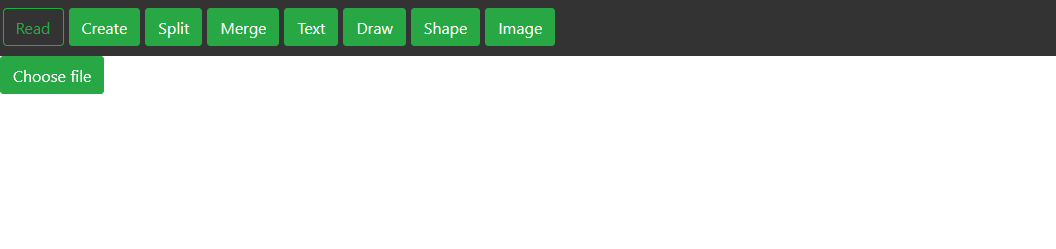
\includegraphics[width=1\textwidth]{"images/startseite.png"}
	\caption{Startseite der PDF Web App}
	\label{fig:start}
\end{figure}

Initial ist der Reader ausgewählt. Ausgewählte Funktionen im Hauptmenü sind dunkelgrau unterlegt mit grüner Schrift. Der Button Create führt zum Creator für leere PDFs, Split zum Splitter fürs Seiten Zerteilen, Merge zum Merger für PDFs zusammenfügen und Text, Draw, Shape bzw. Image öffnen den Editor. Bei Read, Text, Draw, Shape und Image erscheint zunächst der Choose file Button, damit man im Dateisystem ein PDF-Dokument auswählen kann zum Lesen oder Bearbeiten. Klickt man auf Choose file wird der Dateibrowser geöffnet und man kann ein einzelnes PDF auswählen zum Öffnen. Der Screenshot \ref{fig:reader} zeigt den Reader mit geöffneter PDF-Datei.

\begin{figure}[!htb]
	\centering
	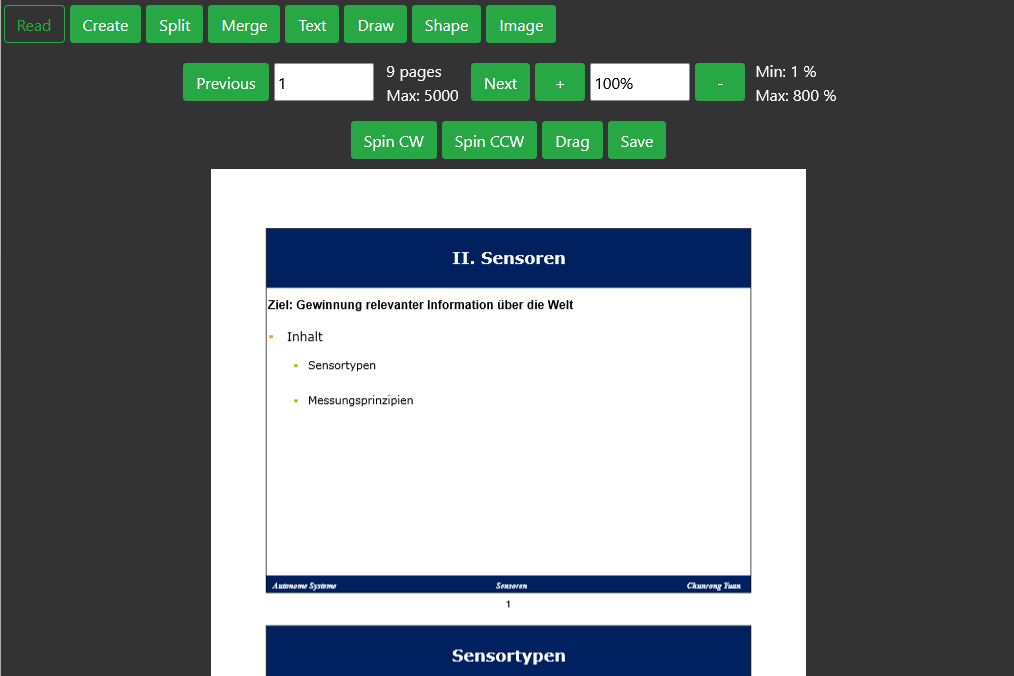
\includegraphics[width=1\textwidth]{"images/reader.png"}
	\caption{Geöffnetes PDF im Reader der PDF Web App}
	\label{fig:reader}
\end{figure}

Falls eine andere Dateiart im Dateibrowser geöffnet wurde erscheint die Fehlermeldung in Screenshot \ref{fig:errorfile}. 

\begin{figure}[!htb]
	\centering
	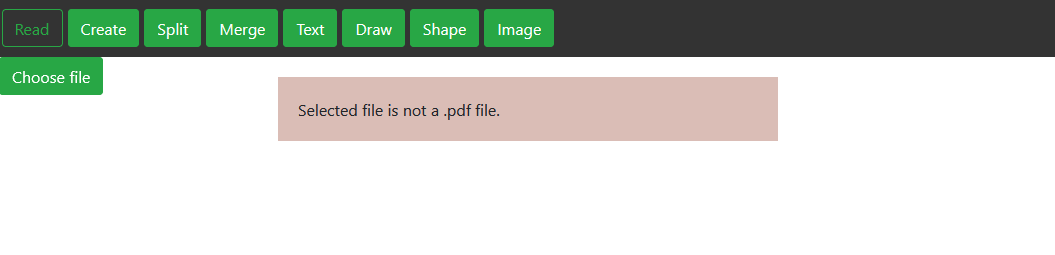
\includegraphics[width=1\textwidth]{"images/errorfile.png"}
	\caption{Fehlermeldung bei einer nicht-PDF-Datei}
	\label{fig:errorfile}
\end{figure}

Auch bei einer verschlüsselten PDF-Datei wird eine im Screenshot \ref{fig:errorcrypt} dargestellte Fehlermeldung angezeigt.

\begin{figure}[!htb]
	\centering
	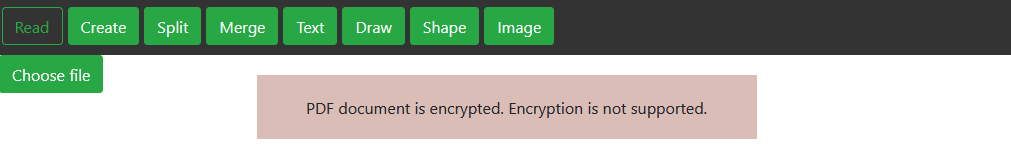
\includegraphics[width=1\textwidth]{"images/errorcrypt.png"}
	\caption{Fehlermeldung bei einem verschlüsselten PDF}
	\label{fig:errorcrypt}
\end{figure}

Bei diesen gezeigten Fehlermeldungen kann man einfach erneut den Dateibrowser aufrufen mit Choose file oder einen anderen Menüpunkt wählen, damit die Fehlermeldung verschwindet. Hat man eine PDF-Datei im Reader geöffnet präsentieren sich einem 2 Zeilen mit Funktionsbuttons. Mittels Previous und Next kann der Benutzer zur vorherigen bzw. nächsten Seite blättern. Zwischen diesen Buttons wird die aktuelle Seite im input field angezeigt und daneben Anzahl an Seiten im Dokument. Im input field kann man eine Seite eingeben und der Reader springt direkt zu dieser Seite. Durch die Buttons Plus und Minus kann man rein- bzw. rauszoomen. Der aktuelle Zoomfaktor wird angezeigt in Prozent und man kann den Zoomfaktor auch mittels Benutzerangabe manuell setzen mit und ohne Prozentzeichen. Spin CW und Spin CCW dreht die aktuelle Seite, die im input field angezeigt ist, um 90 Grad im Uhrzeigersinn (clockwise) und gegen den Uhrzeigersinn (counterclockwise). Durch die Funktion Drag kann man die aktuelle Seite verschieben im Viewport. Das ist nützlich, wenn man an das PDF nah rangezoomt hat und die Seite nur teilweise sehen kann. Der Save Button downloaded das aktuelle PDF im Downloads-Ordner des Benutzers. \\

Der Creator ist mittels Create Buttons im Hauptmenü aufrufbar. Im Screenshot \ref{fig:creator} ist die GUI vom Creator dargestellt. 

\begin{figure}[!htb]
	\centering
	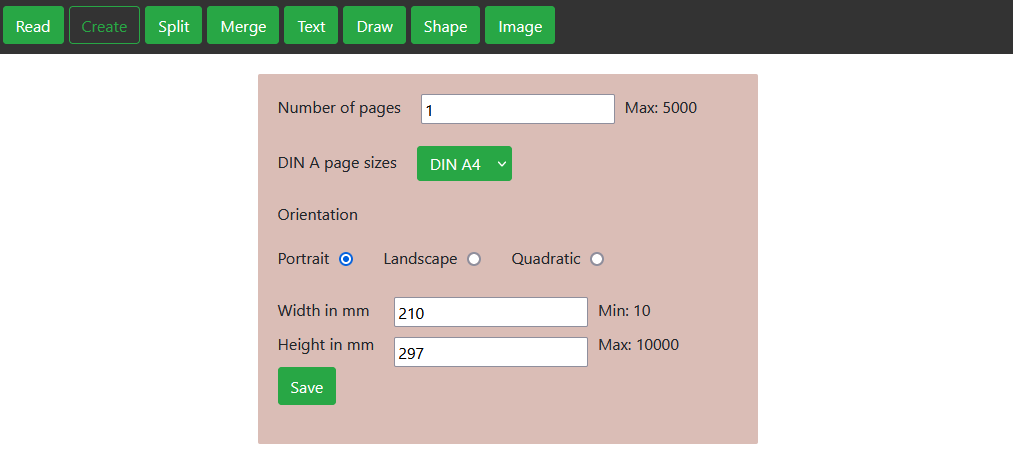
\includegraphics[width=1\textwidth]{"images/creator.png"}
	\caption{Creator GUI der PDF Web App}
	\label{fig:creator}
\end{figure}

Man gibt eine Anzahl an gewünschten Seiten des leeren PDFs ein und die Breite und Höhe in mm. Wahlweise kann man den Selector verwenden um ein DIN A-Preset zu verwenden. Mittels der Schnellauswahl kann man die Orientierung bestimmten: Portrait, Landscape oder Quadratisch. Der Save Button downloaded das leere PDF. \\
Zum Splitter kann man mit dem Split Button gelangen, der vom Screenshot \ref{fig:splitter} gezeigt wird.

\begin{figure}[!htb]
	\centering
	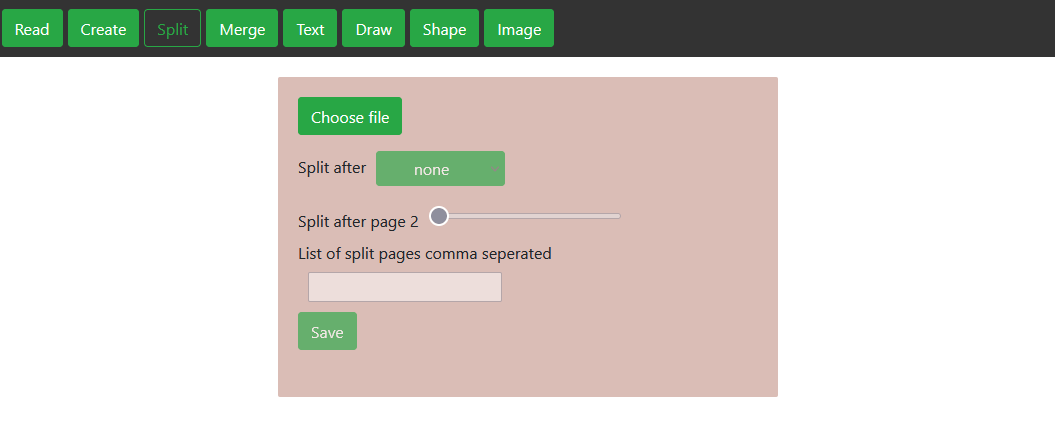
\includegraphics[width=1\textwidth]{"images/splitter.png"}
	\caption{Splitter GUI der PDF Web App}
	\label{fig:splitter}
\end{figure}